\documentclass[sigconf]{acmart}

\usepackage{booktabs} % For formal tables
\usepackage{balance}
% Copyright
%\setcopyright{none}
%\setcopyright{acmcopyright}
%\setcopyright{acmlicensed}
%\setcopyright{rightsretained}
%\setcopyright{usgov}
%\setcopyright{usgovmixed}
%\setcopyright{cagov}
%\setcopyright{cagovmixed}

\usepackage{multirow}

\usepackage{comment}

% DOI
%\acmDOI{10.475/123_4}

% ISBN
%\acmISBN{123-4567-24-567/08/06}

%Conference
%\copyrightyear{2021} 
%\acmYear{2021} 
%\setcopyright{acmcopyright}
%\acmConference[SIGCSE '21]{Proceedings of the ACM Technical %Symposium on Computer Science Education}
%\acmBooktitle{Proceedings of the ACM Technical Symposium on Computer Science Education (SIGCSE '21)}
%\acmPrice{15.00}
%\acmDOI{10.1145/3287324.3287496}
%\acmISBN{978-1-4503-5890-3/19/02}


\newcommand{\gameNameNS}{``Game Name''}
\newcommand{\gameName}{\gameNameNS~}
\newcommand{\pwOne}{\gameName \emph{v.}1.0~}
\newcommand{\pwOneNS}{\gameName \emph{v.}1.0}
\newcommand{\pwTwo}{\gameName \emph{v.}2.0~}
\newcommand{\pwTwoNS}{\gameName \emph{v.}2.0}
\newcommand{\pwThree}{\gameName \emph{v.}3.0~}

\newcommand{\JA}[1]{\footnote{\textbf{JA: #1}}}

% Programming Cards
\newcommand{\I}{\texttt{Instruction~}}
\newcommand{\Ins}{\texttt{Instruction}}
\newcommand{\M}{\texttt{Method~}}
\newcommand{\Mns}{\texttt{Method}}
\newcommand{\Gr}{\texttt{Group~}}
\newcommand{\Grns}{\texttt{Group}}
\newcommand{\R}{\texttt{Repeat~}}
\newcommand{\Rns}{\texttt{Repeat}}
\newcommand{\Rx}{\texttt{Repeat-X~}}
\newcommand{\Rxns}{\texttt{Repeat-X}}
\newcommand{\V}{\texttt{Variable~}}
\newcommand{\Vns}{\texttt{Variable}}

\newcommand{\Ser}{\texttt{Search~}}
\newcommand{\Serns}{\texttt{Search}}
\newcommand{\Sort}{\texttt{Sort~}}
\newcommand{\Sortns}{\texttt{Sort}}

%Safety
\newcommand{\Anti}{\texttt{Antivirus~}}
\newcommand{\Antins}{\texttt{Antivirus}}
\newcommand{\Scan}{\texttt{Computer Scan~}}
\newcommand{\Scanns}{\texttt{Computer Scan}}
\newcommand{\Fire}{\texttt{Firewall~}}
\newcommand{\Firens}{\texttt{Firewall}}
\newcommand{\Over}{\texttt{Overclock~}}
\newcommand{\Overns}{\texttt{Overclock}}


% Malware
\newcommand{\Vi}{\texttt{Virus~}}
\newcommand{\Vins}{\texttt{Virus}}
\newcommand{\Ran}{\texttt{Ransomware~}}
\newcommand{\Ranns}{\texttt{Ransomware}}
\newcommand{\Spy}{\texttt{Spyware~}}
\newcommand{\Spyns}{\texttt{Spyware}}
\newcommand{\Trj}{\texttt{Trojan Horse~}}
\newcommand{\Trjns}{\texttt{Trojan Horse}}
\newcommand{\Mal}{\texttt{Malware~}}
\newcommand{\Malns}{\texttt{Malware~}}

% Hacking
\newcommand{\Hack}{\texttt{Hack~}}
\newcommand{\Hackns}{\texttt{Hack}}
\newcommand{\Buf}{\texttt{Buffer Overflow~}}
\newcommand{\Bufns}{\texttt{Buffer Overflow}}
\newcommand{\CSS}{\texttt{Cross-site Scripting~}}
\newcommand{\CSSns}{\texttt{Cross-site Scripting}}
\newcommand{\SQL}{\texttt{SQL Injection~}}
\newcommand{\SQLns}{\texttt{SQL Injection}}
\newcommand{\DoS}{\texttt{Denial of Service~}}
\newcommand{\DoSns}{\texttt{Denial of Service}}



% Areas
\newcommand{\MS}{\emph{Method Stack~}}
\newcommand{\MSns}{\emph{Method Stack}}
\newcommand{\Play}{\emph{Main~}}
\newcommand{\Playns}{\emph{Main}}
\newcommand{\Bns}{\emph{Bonus~}}
\newcommand{\Bnsns}{\emph{Bonus}}

\newcommand{\Hand}{\texttt{Player's Hand}}
\newcommand{\Prg}{\texttt{Program Editor}}
\newcommand{\Hist}{\texttt{Game History}}
\newcommand{\Goals}{\texttt{Gameplay Goals}}




% Modes
\newcommand{\B}{\emph{Beginner~}}
\newcommand{\BNS}{\emph{Beginner~}}
\newcommand{\Std}{\emph{Standard~}}
\newcommand{\StdNS}{\emph{Standard}}



\begin{document}

\settopmatter{printacmref=true}
\fancyhead{}

\title{Need a tittle}
%\titlenote{Produces the permission block, and
%  copyright information}
%\subtitle{A Card Game for Teaching Cybersecurity, Algorithms and Methods}
\subtitle{************************}
%A Game-based Approach to Teaching Programming and Cybersecurity Concepts}
%\subtitle{Applying Game-based Learning for Teaching Programming and Cybersecurity Concepts}
%\subtitle{Learning Basic Programming and Cybersecurity Concepts through a Game-based Approach}



%\subtitlenote{The full version of the author's guide is available as
  %\texttt{acmart.pdf} document}

\author{Anonymized Author(s)}



%\author{John Anvik$^*$,\hspace{0.5em} Md. Hasan Tareque$^*$,\hspace{0.5em} Steven Deutokom$^*$ ,\hspace{0.5em} Maimoona Bashir$^*$ }
%\affiliation{%
% \vspace{0.5em}\institution{University of Lethbridge$^*$}
%}
%\affiliation{%
%  \institution{\{john.anvik,\hspace{0.2em}mdhasan.tareque,\hspace{0.2em}deutekom,\hspace{0.2em}maimoona.bashir\}@uleth.ca}
%}

% 
% % The default list of authors is too long for headers.
%\renewcommand{\shortauthors}{Anvik et al.}

\begin{abstract}
Need to re-write.

\end{abstract}

%
% The code below should be generated by the tool at
% http://dl.acm.org/ccs.cfm
% Please copy and paste the code instead of the example below.
%
\begin{CCSXML}
	<ccs2012>
	<concept>
	<concept_id>10010405.10010489.10010491</concept_id>
	<concept_desc>Applied computing~Interactive learning environments</concept_desc>
	<concept_significance>500</concept_significance>
	</concept>
	<concept>
	<concept_id>10003456.10003457.10003527.10003528</concept_id>
	<concept_desc>Social and professional topics~Computational thinking</concept_desc>
	<concept_significance>300</concept_significance>
	</concept>
	<concept>
	<concept_id>10003456.10003457.10003527.10003531.10003533.10011595</concept_id>
	<concept_desc>Social and professional topics~CS1</concept_desc>
	<concept_significance>300</concept_significance>
	</concept>
	<concept>
	<concept_id>10003456.10003457.10003527.10003539</concept_id>
	<concept_desc>Social and professional topics~Computing literacy</concept_desc>
	<concept_significance>300</concept_significance>
	</concept>
	</ccs2012>
\end{CCSXML}

\ccsdesc[500]{Applied computing~Interactive learning environments}
\ccsdesc[300]{Social and professional topics~Computational thinking}
\ccsdesc[300]{Social and professional topics~CS1}
\ccsdesc[300]{Social and professional topics~Computing literacy}

\keywords{Programming language education; Cybersecurity education; Web application; Card game; Game-based Learning}

\maketitle
\section{Introduction}

***Needs to update.***

Most games and environments developed with the intention of teaching computer programming concepts do so by requiring the student to either learn an existing programming language (e.g. Java \cite{Robocode}, Python \cite{CodeWars,CheckIO} or JavaScript \cite{CodeCombat,CheckIO,Codingame}) or a language specific to the learning environment (e.g. Scratch \cite{Scratch} or Alice \cite{Alice}). If the goal is to teach the fundamental concepts of computer programming, this requirement can result in a situation where the learner feels intimidated, confused or frustrated when their ``program'' does not work correctly. Also, as Bromwich et al. noted, many of these educational programming languages and environments are ``often ambitious in what they are trying to teach beginning programmers. They even go as far as to try teaching concurrency, something with which even advanced programmers often have difficulty.'' \cite{Bromwich2012}.

Also, such learning games and environments commonly use either a puzzle-solving premise, such as navigating a maze, or a sandbox paradigm, where a learner can utilize the language in an open-ended manner. As puzzle-solving activities tend to favour a specific demographic \cite{Phan2012}, and the sandbox paradigm requires oversight by an outside influence (i.e. an instructor) to ensure learning progression \cite{Bromwich2012}, both approaches have significant drawbacks.    

\gameNameNS
%\footnote{https://github.com/SibylLab/program-wars}
\footnote{Project repository URL removed for blind-review.} 
was created to address these concerns by providing a web-based card game that teaches or reinforces the fundamental concepts of programming and cybersecurity to those with limited or no programming or computer security experience \cite{anvikPW}. Players use various cards to create a program that executes a target number of instructions while launching cyberattacks against opponents and using representations of cybersecurity tools to defend themselves. Players are awarded additional points according to how they construct their program.

Several limitations and areas for improvement were identified for the initial version of \gameName following both formal \cite{anvikPW} and informal observations and discussions with players. The specific limitations identified included: confusion regarding the concept of method/function/procedure, the overgeneralization of cyberattacks, and frustration due to the randomness of the ``conditional statement" game mechanic.

This paper presents a redesign of \gameName which addresses these limitations, resulting in \pwTwoNS, a version which we believe better communicates the principles of functional decomposition, conditional statements, and real-world cybersecurity concepts. Also, \pwTwo introduces learners to two key classes of algorithms: searching and sorting.

The paper proceeds by presenting a survey of card or board games whose intent is similar to that of \gameName, followed by a description of the gameplay and cards found in \pwTwoNS.

\section[Related Work]{Related Work}
\label{sec:Related Work}

There are several research works have been conducted regarding the use of games for teaching computer programming and software engineering.

\subsection{Game-Based Learning research in SE}
The following is an overview of the previous work regarding Game-Based Learning in the field of software engineering.

Tao et al. \cite{educational} emphasize learning software engineering through different gaming approaches. In their research, they found that gaming for software engineering education required a slightly different approach than the traditional Game-Based Learning methodologies. They created Pex4Fun to serve both the social aspects of Game-Based Learning and the presentation of software engineering content. The learning outcome from the research work is gaming and entertainment can be a source of education and that interactive learning has excellent value. Another discovery is that learning while playing can be effective in the industrial field.

Swapneel et al. \cite{halo} discussed how highly addictive socially optimized (HALO) provides concentration through an adaptive environment. The game environment is developed in such a way so that the player can enjoy the work in a gaming atmosphere. The initial stage is known as ‘Quest’, which is a preliminary introduction of the system. Here someone senior must work voluntarily or can be assigned. If the quest is harder for a single player, it could be done in a team, and then it is called a party. Another essential aspect is context switching. If an employer works on different modules then it will require more time, but HALO groups the same type of coding all together so that less context switching is required. Both the academic and industrial fields can be beneficial by adopting the game-based approach in software engineering.  Evaluation of the technique was not present, which is one of the drawbacks of this research.  

Miljanovic et al. \cite{robobug} discussed Robobug, a debugging technique through gaming in their research paper. Debugging is an essential tool in programming. Many good programmers struggle to find the bugs in a code segment. Debugging requires practice and patience; both might be difficult for a new programmer. Many computer science students struggle with debugging and feel left behind. Robobug presents different debugging techniques at different levels.

Szabo \cite{gamedev} proposed GameDevTycoon for teaching software engineering. Based on their work, there are thirteen different criteria for Game-Based Learning. GameDevTycoon covers most of the criteria. Gameplay analysis and software process models are simultaneously covered in the game. Three primary stages of software development are taught through the gameplay. The initial stage is known as the garage, the second stage is called team management, and the final stage is known as world domination. Each stage has separate responsibilities; for example, in the initial stage in software development, one should focus on the quality and latest research.

Pieper et al. \cite{SEMAT} presented a case study of the Software Engineering Method and Theory (SEMAT) to identify the educational outcomes in Digital Game-Based Learning. SEMAT is a part of the emerging OMG\footnote{The Object Management Group (OMG) is a computer industry standards consortium.} standard \cite{kernerl}. The case study shows that the evaluation of a developed integrated scenario can provide an in-depth analysis of the result. Nevertheless, the data was not sufficient to reach a conclusive decision regarding the pattern of learning. As a result, SEMAT was not referred to as a standard.

Mauricio et al. \cite{gamesforlearning} identified a different methodology that can be or is already applied in different interactive games for Software Engineering (SE) Game-Based Learning. Also, they explored different primary studies related to SE education, found the learning outcomes and mapped those outcomes to different SE project stages. 

Vladimir et al. \cite{gamification} discussed the different classifications of gameplay and their impact on several learning criteria. According to the researchers, gamification is a growing area in the business industry. The researchers emphasized the SWOT (Strengths, Weaknesses, Opportunities, Threats) framework \cite{swot} to find the learning criteria. However, they found that creating a software engineering Game-Based engine is a challenging task, one which programmers and industry should give a high priority. 

\begin{comment}

\subsection{Games for Learning Software Engineering}
Several games have been created for teaching the basics of programming and software engineering. However, most of them are platform-oriented (i.e. only work on Windows) or target a specific programming language (e.g. C++ or Java). For learning the basics regarding computer programming and SE, it is essential to understand the underlying logic and conceptual ideas. There are some games related to the learning. 


\subsubsection{Board Games}
Board games are a part of tabletop games where different components of the game can be moved on an adjacent surface or board according to some predefined rules.

Battle Bots v2 \cite{BattleBotsv2}  was inspired by the Robo Rally \cite{roborally} game. The required number of players for the game is between two and twenty. In the middle of the board, there is a repair center. Each player will start the game with twenty-two cards. Each move is divided into two groups: the programming round and the action round. In the programming round, players have to play the movement cards. In this stage, no action card can be played. In action round, there are five-phase where different action cards can be played along with movement cards. The player who survives the match wins the game. The main advantage of the game is that the players have to plan about the moves, which is an important programming concept, as in software development.


Robot Turtles \cite{RobotTurtles} is a game to teach kids to code by using simple direction cards to move a specific coloured turtle. The main focus of the game is to get the coloured turtle to the same coloured jewel piece on the board. There are three instructions: forwards, rotate 90 degrees left and rotate 90 degrees right. There are also some obstacles where players might have to use different techniques to overcome the situation, and some unique cards are also introduced like fire cards for shooting. The higher the level, the more complex cards need to be used.
Regarding programming, the jump card is the most crucial one. The idea of jump cards is that they can be replaced with a set of instruction cards that can be used repeatedly. There is also a bug card that can undo the immediate move the player has made which is important in SE development.


Code Master \cite{CodeMaster} is a single person puzzle game that teaches logical problem-solving. There are sixty levels in the game with several challenging levels. The game consists of a map that has six different levels ranging from easy (green) to expert (red). There is also a guide scroll that indicates the order in which the program statements should run. The game focuses on the programming construct of conditional statements (i.e. if-else). Some nodes have a self-loop, which illustrates the concept of a repeat statement. Finally, the shortest path selection is also a focus point. The game requires essential thinking before each move, which is vital for developing logical thinking. 

\subsubsection{Card Games}

A card game can be defined as a game that involves different playing cards as the main components with which the game can be played.

Potato Pirates \cite{PotatoPirates} was the only physical card game found that intends to teach programming concepts. The main objective of the game is to make the user familiar with different programming concepts through social interactions. The final goal of the game is to achieve seven specific cards, named Potato King, through different logical actions performed through different cards. To win the game, a player needs to eliminate all the other ships in possession of the other players or acquire all seven Potato Kings by drawing them from the deck or by eliminating other players’ ships and seizing their cards. Players can power up their attacks with programming concepts cards such as loops and conditionals. The game covers the concepts of programmings such as variables, functions, while-loops, if-else conditionals and nested-loops. Some surprise cards serve the purpose of interrupts and control flow. The game illustrates the branching condition very nicely, which is equivalent to the if-else statement. The use of variables is well defined. Different repeat structures are also presented in a reasonable manner such that the game covers the loop structure of programming languages. There is also an option for creating a loop inside a loop, which is known as a nested loop. The game also covers the case structure (switch case or nested if-else).

\subsubsection{Web-based Games}

Games that can be played on the World Wide Web are known as web-based games. These games use standard web technologies or browser plugins \cite{webbasedgames}.

CodeCombat \cite{CodeCombat} is a web-based game focusing on learning JavaScript, Python, and other programming languages. The game is built upon concepts of swords-and-sorcery where the player has to role-play as a warrior. The main objective of the game is to learn necessary programming skills by overcoming different challenges like clearing the maze, picking up gems and avoiding any spikes or attacking ogres. The gameplay is split between a code editor on the right and a simulation effect on the left. Figure \ref{fig:CodeCombat} shows the interface of the game. The avatar is controlled by using a set of commands.  In each level, the player has to accomplish a set of tasks. As the game progresses, the player is gradually introduced to new concepts like loops, conditionals, and variables. If a person does not have programming experience, CodeCombat is very suitable. As the game progresses, the tasks involve more complex programming concepts. Most importantly, the levels themselves become more complicated due to possible interactions with the objects in the game world.\\

\begin{figure}[ht!]
	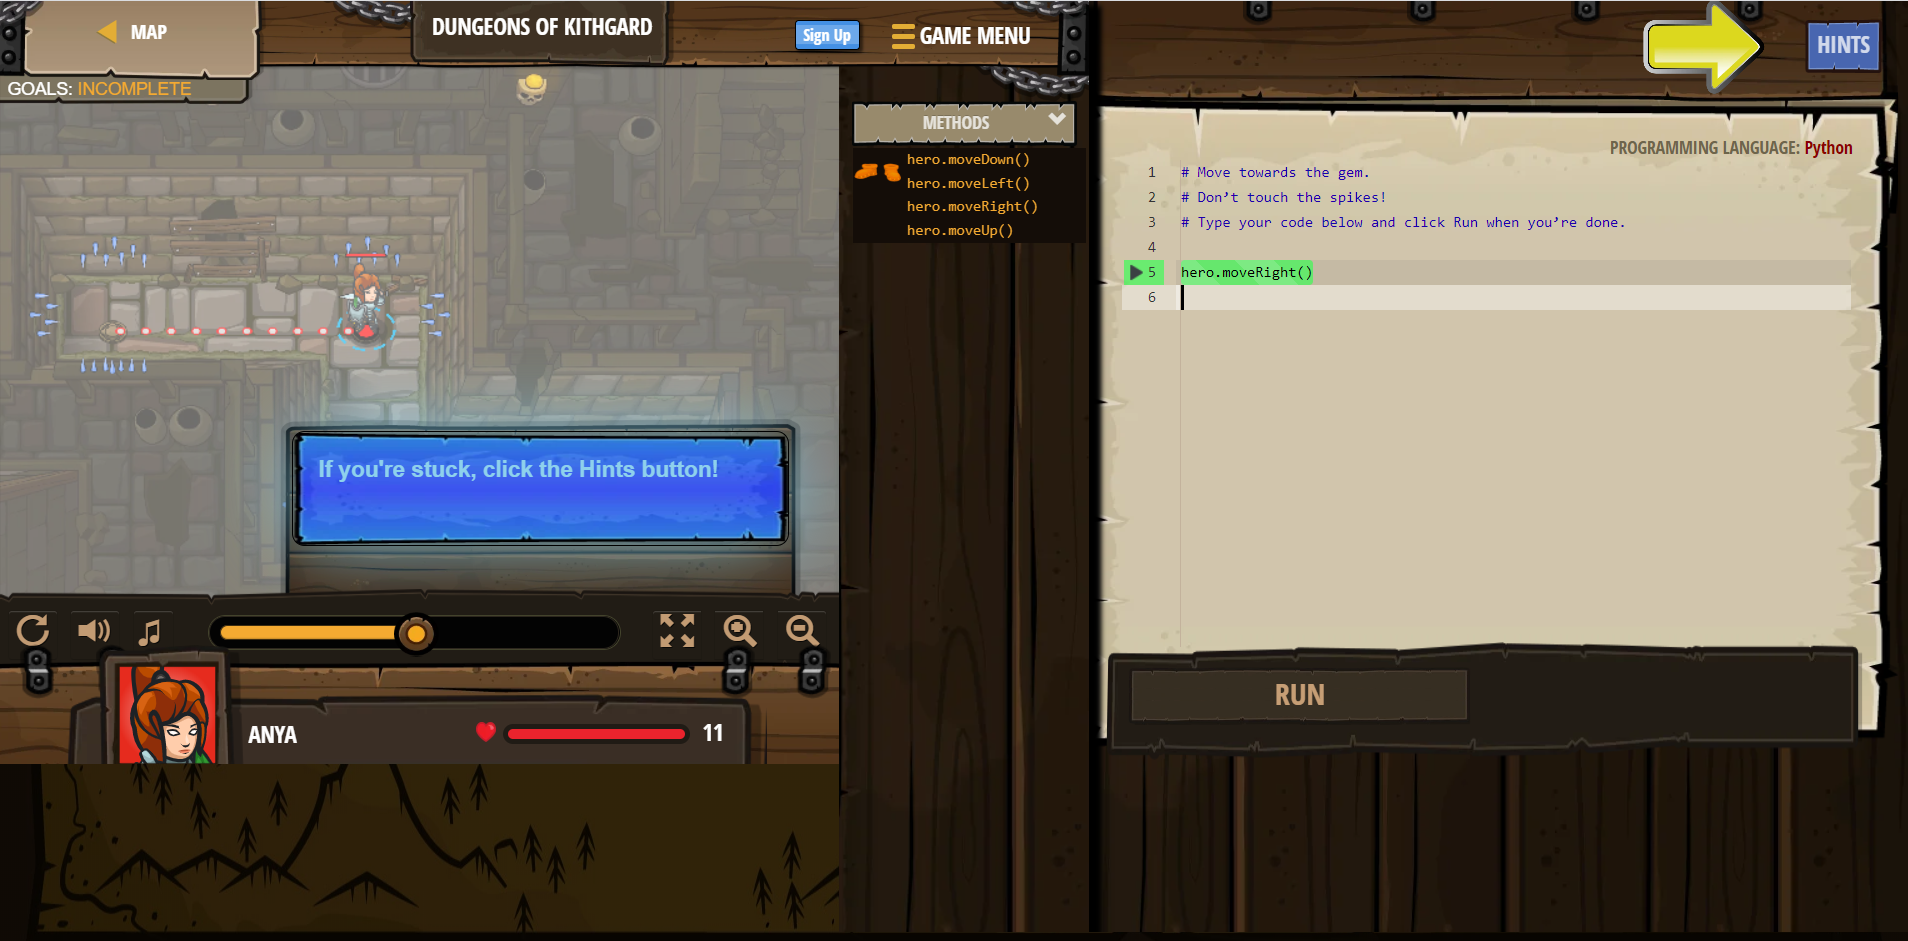
\includegraphics[width=\columnwidth]{images/CodeCombat.PNG}
    \caption{CodeCombat gameplay}
    \label{fig:CodeCombat}
\end{figure}


Blocky maze \cite{Blocklymaze} is a game that introduces the concept of programming loops and conditions in Javascript without writing any Javascript code. The game is a combination of levels that teach programming. It is designed for children who have not had prior experience with computer programming. The game uses a graphical programming language implemented in JavaScript, which can compile to JavaScript, Dart or Python. In the game, programming is done by dragging and dropping code blocks onto a design surface. Figure \ref{fig:BlocklyMaze} shows the interface of the game. The main objective of the game is to take the avatar from a starting point to the endpoint. There are a total of ten levels, and the complexity increases as the game progress. Some goals are set to solve the maze in a particular number of steps, which is also challenging. The game interface is similar to a Google Map, which might help the user to adopt the game. 

\begin{figure}[ht!]
	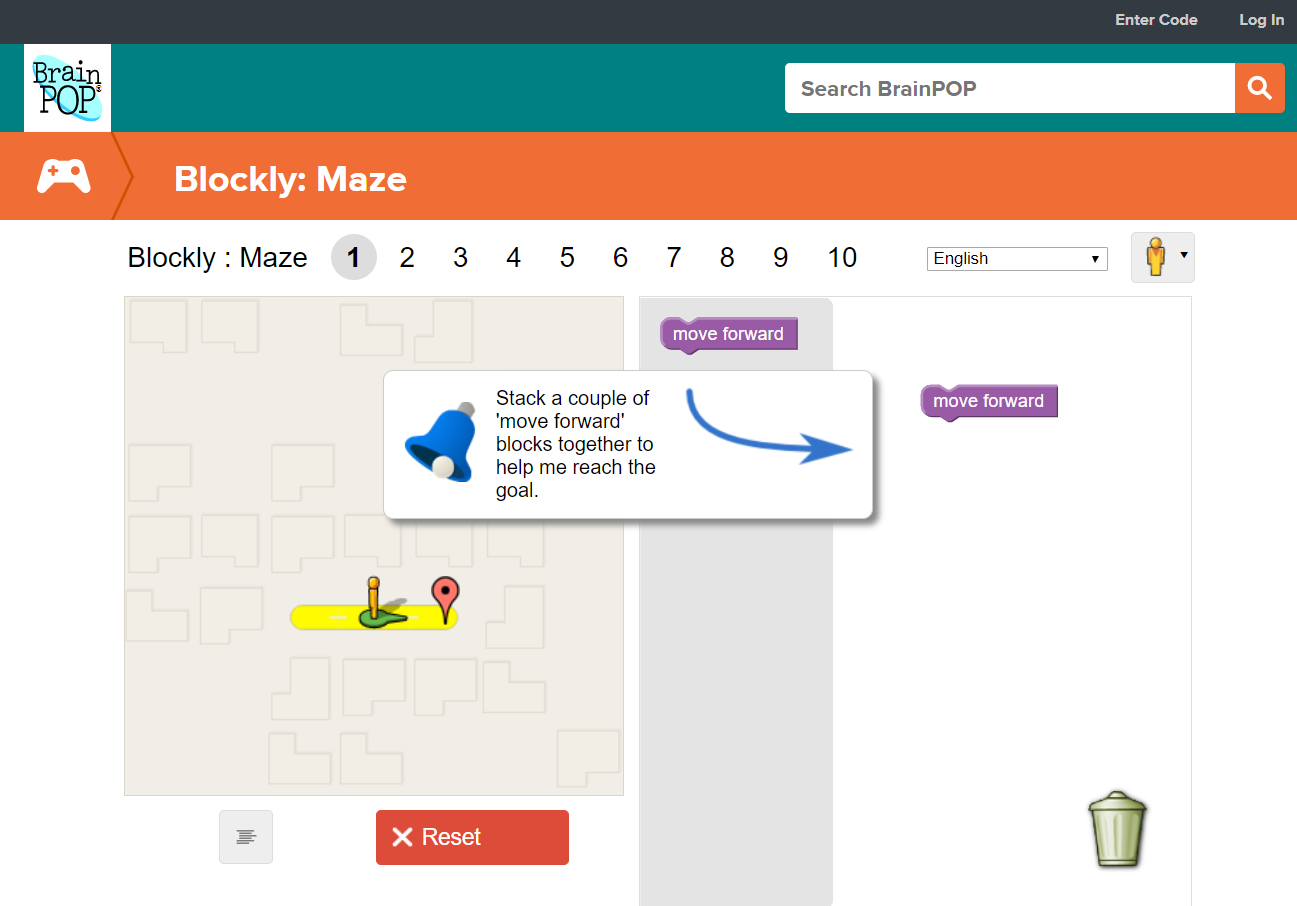
\includegraphics[width=\columnwidth]{images/BlocklyMaze.PNG}
    \caption{Blockly Maze gameplay}
    \label{fig:BlocklyMaze}
\end{figure}

CodinGame \cite{Codingame} supports many programming languages. The main objective of the game is to improve players’ coding skills by solving different problems, applying new strategies and getting inspired by other strong opponents. The game can be played in single and multiplayer mode, which gives it the feeling of fun rather than learning. A player can choose any programming language among more than twenty, such as Python, Ruby, Java, and Scala. The targeted group for the game is the people who have basic programming knowledge as well as expert developers. In the game, users create a profile, which is used for challenges and contests. There are opportunities for players to make their profile public so that employers can find them to offer them a job. Also, the game has a forum for members to chat about languages, questions, and share information. The game is not for beginners because it requires some basic knowledge of programming. Figure \ref{fig:CodinGame} shows the interface of the game.

\begin{figure}[ht!]
	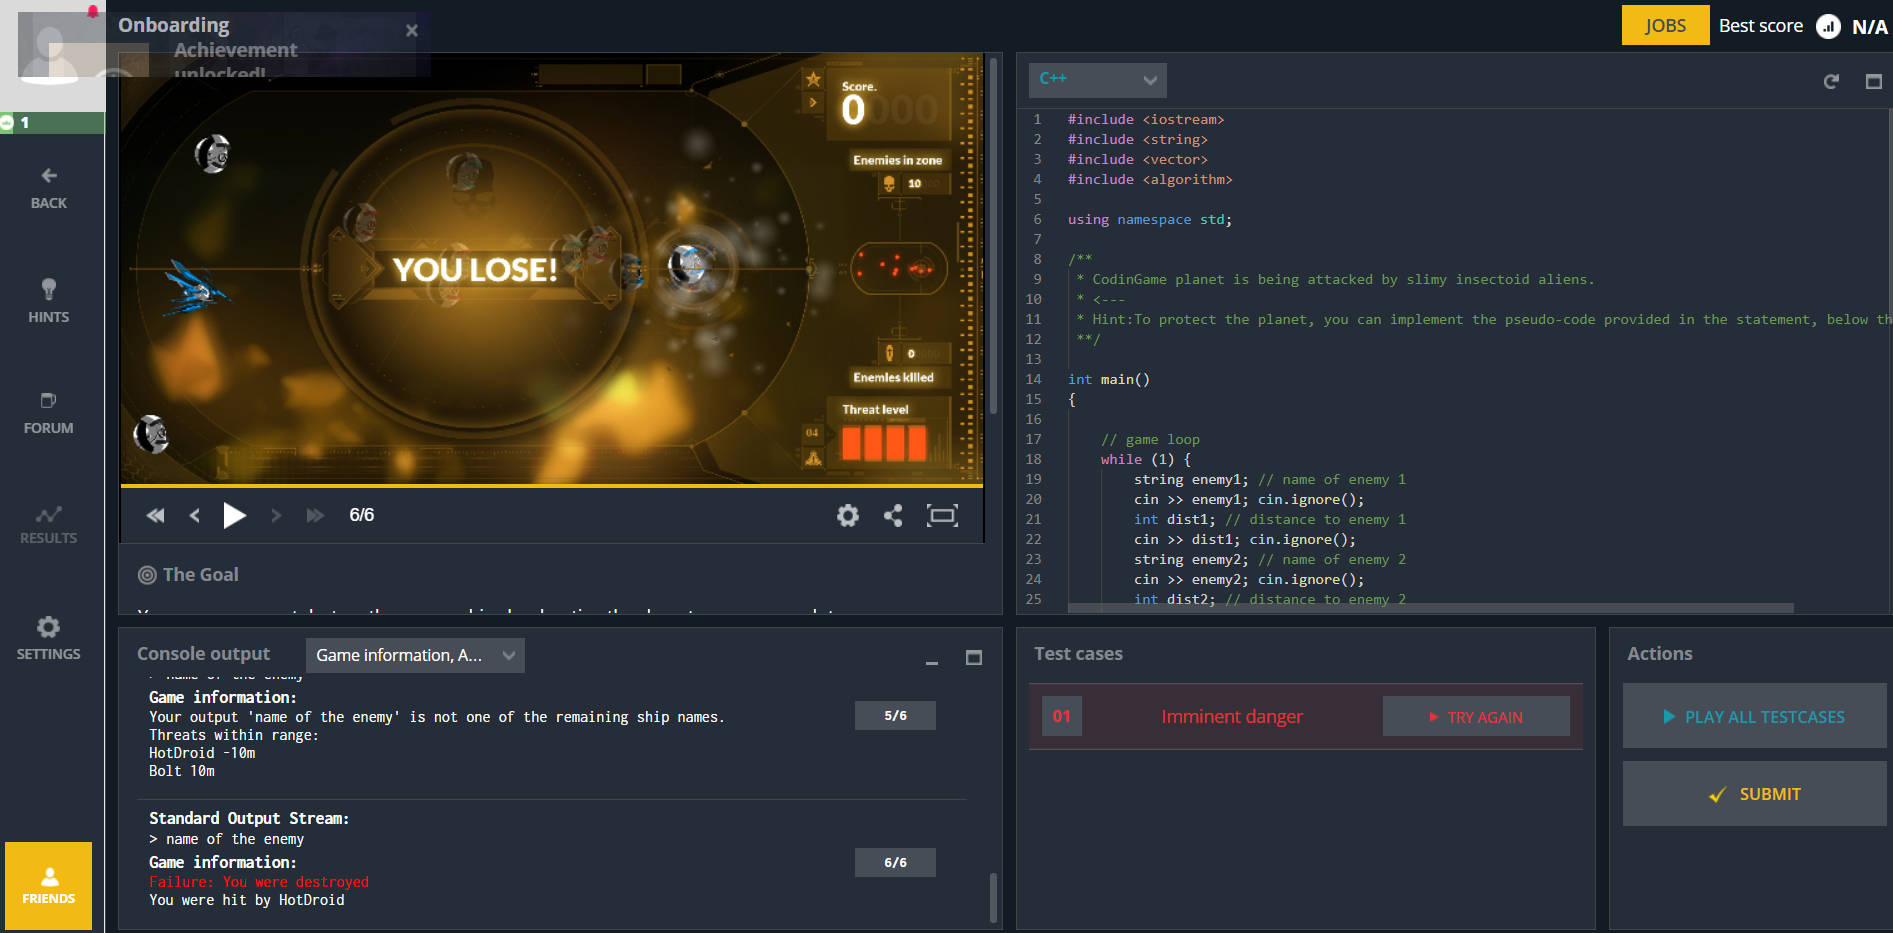
\includegraphics[width=\columnwidth]{images/CodinGame.PNG}
    \caption{CodinGame gameplay}
    \label{fig:CodinGame}
\end{figure}

\begin{figure}[hbt!]
  	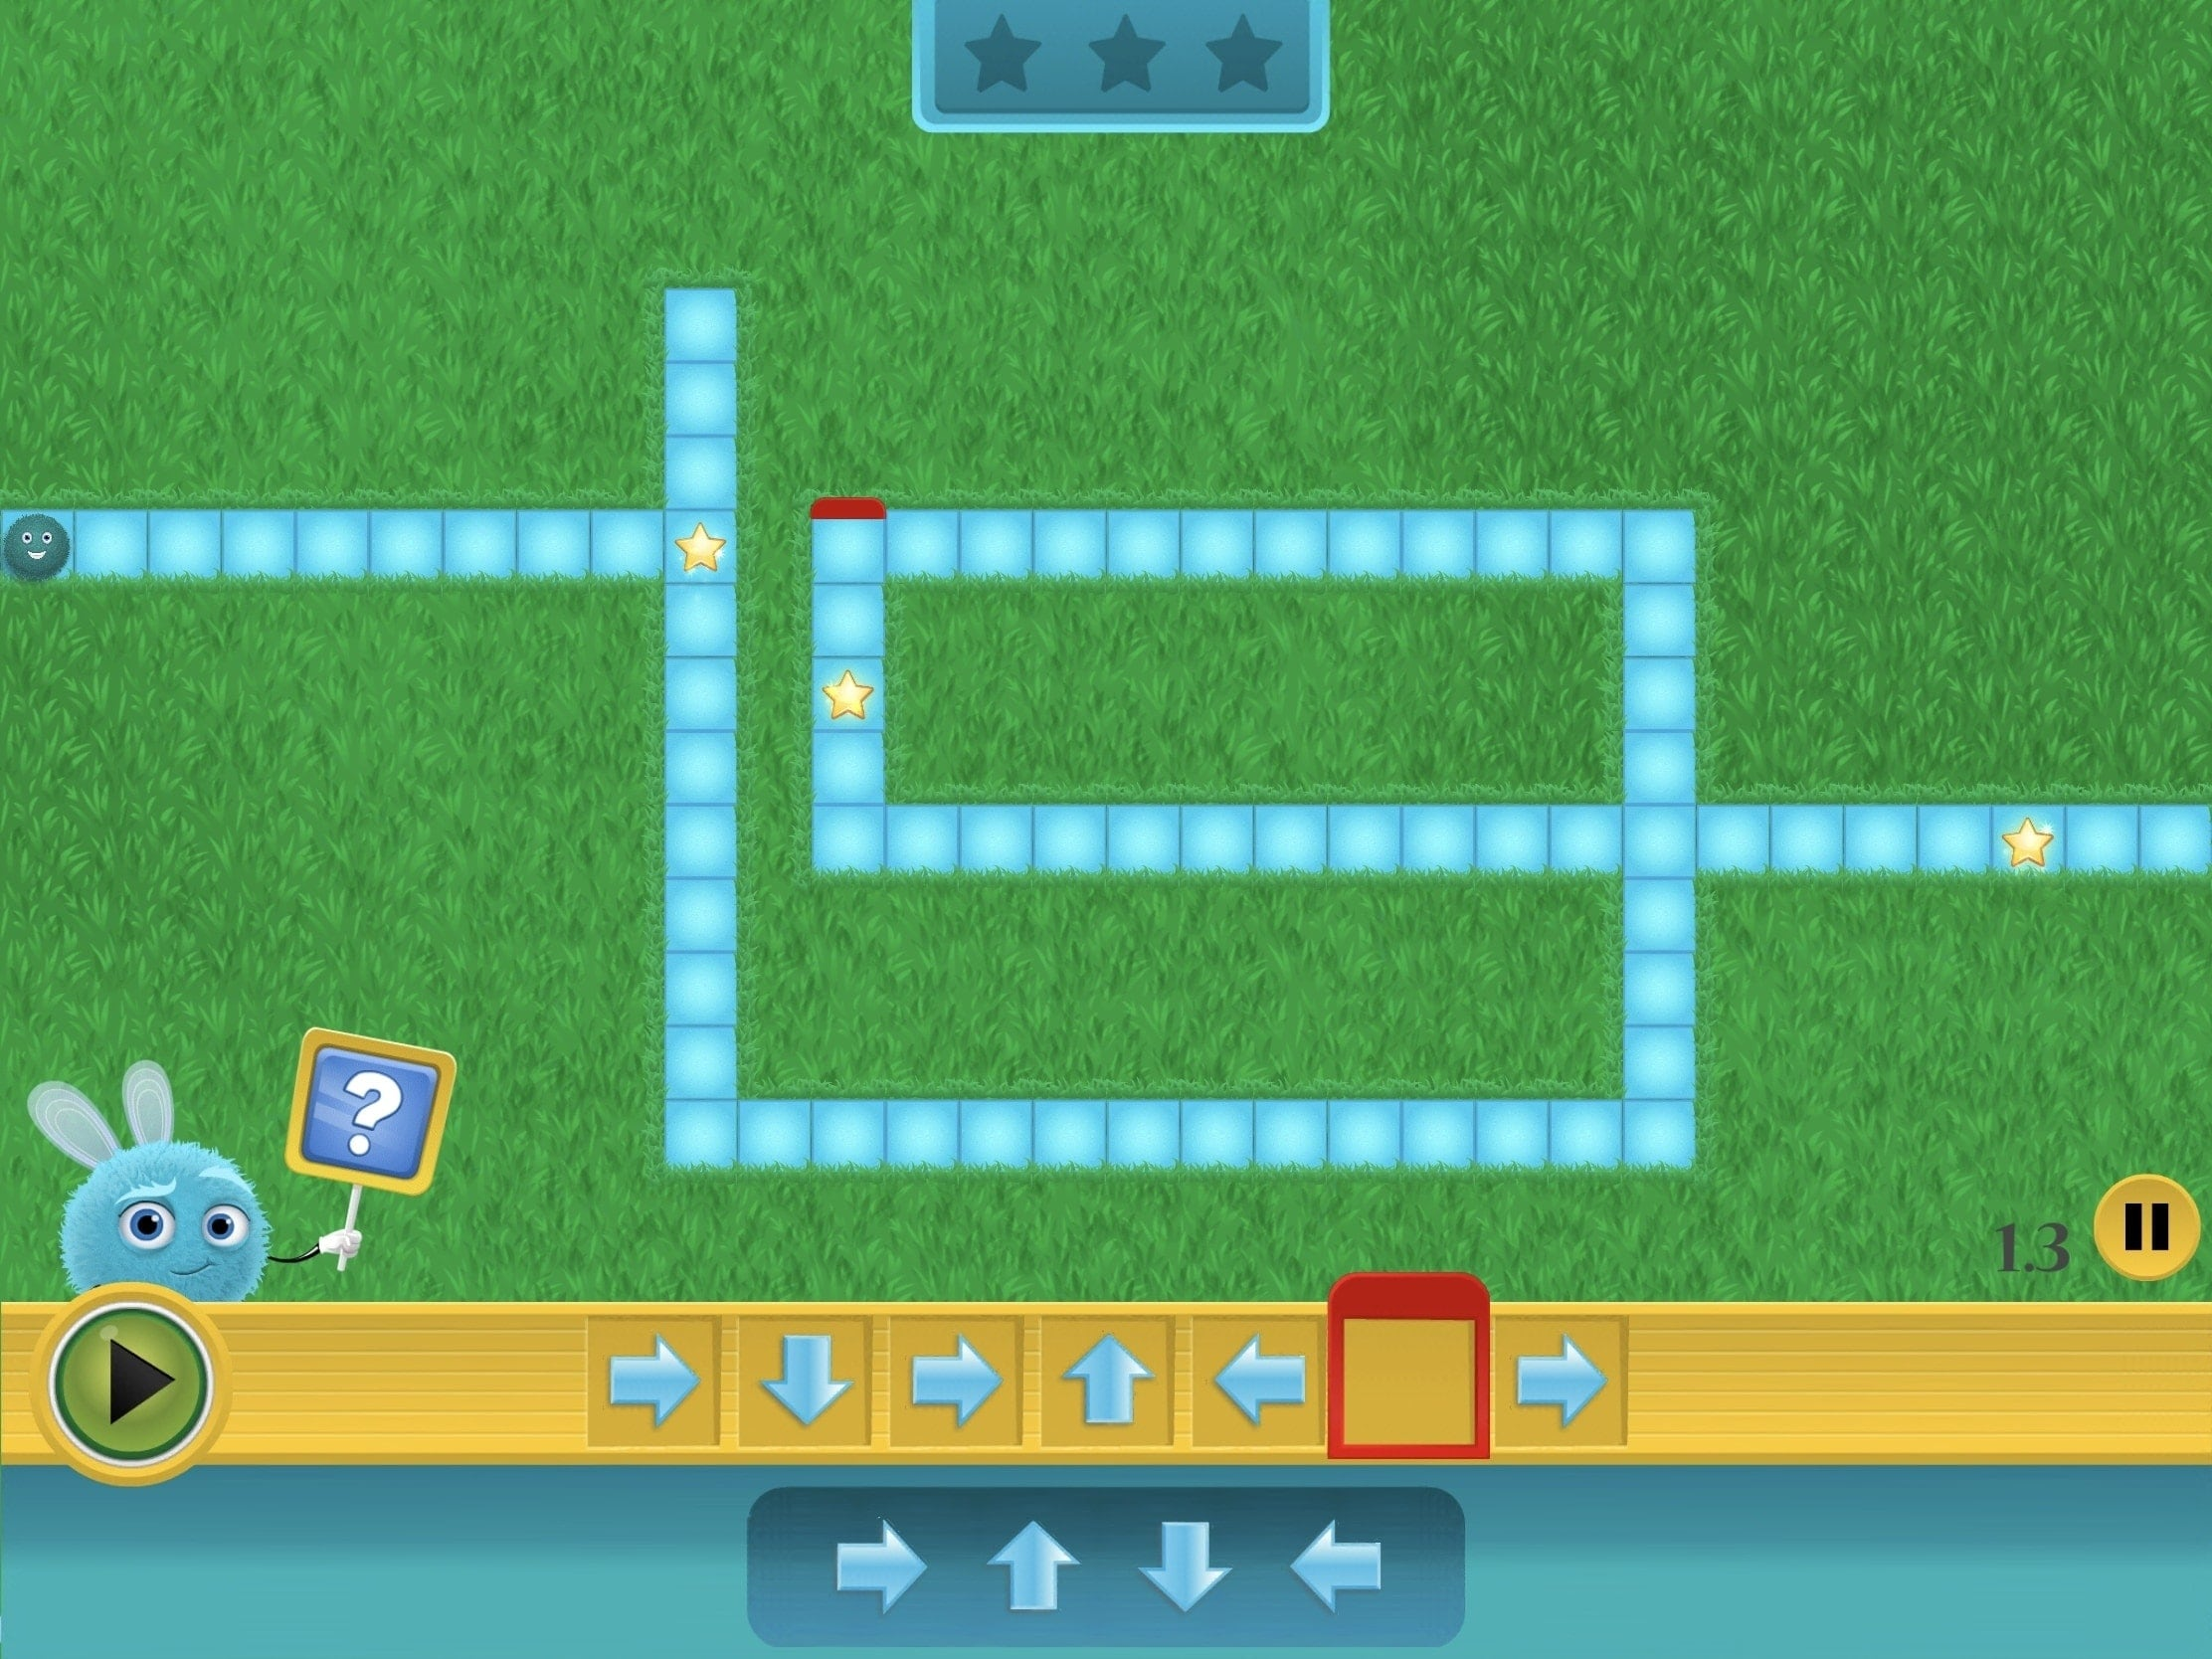
\includegraphics[width=\columnwidth]{images/Kodable.PNG}
    \caption{Kodable gameplay}
    \label{fig:Kodable}
\end{figure}

Kodable \cite{Kodable} is a game developed for kids that focuses on introducing logic and the decisions (i.e. if-then-else) in computer programming. Kodable’s programming language introduces players to step-by-step statements with different instructions using in the programming language. The primary programming concepts of conditional statements and loop structure, is well defined in the game. The social aspect of the game is presented into a parents section with written teaching instructions that assist the parent to unlock different levels for kids and extend logic skills into real life. The game is comprised of many features that are appropriate for children. The activities in the game help the player to think like a programmer, solve different problems and eventually to writing real code using the game’s custom coding interface. Figure \ref{fig:Kodable} shows the interface of the game. For logic development, the game focus on learning the importance of statement sequence. The game introduces kids to different types of data, such as integers and strings, and data structures, such as arrays. Finally, object-oriented programming concepts are also introduced by the game. 


Program Wars \cite{ProgramWars} is a web-based card game. The game focuses on learning programming and cybersecurity concepts. The player’s objective is to achieve a specific number of points through different cards. The game is platform-independent, which means that it is not focused on any single programming language. Instead, the game helps to develop an understanding of the underlying logic of programming. Here the players do not have to be concerned about syntax errors, and programming terms are being described using an elementary vocabulary. In Chapter \ref{ch:Overview of Program Wars}, a more detailed analysis regarding Program Wars is presented.   

\end{comment}

%\section{Summary}
%Based on the related research works examined, practical implementation (i.e. learning a real programming language) and visualization of program results are essential in software engineering education. Also, learning through gameplay has more sustainable effects\cite{effectivenessofgames}. The main challenge of Game-Based Learning for software engineering is to maintain a balance between learning and engagement \cite{educationalgamedesign}. The gameplay should be presented in a structured way such that the user can relate the outcome to real-world programming. Most of the research deals with a specific part of a software engineering like debugging, the user interface, and project management.


\section{\pwThree Gameplay Additions}

This section describes the changes and additions \emph{Agile} mode brings to \pwThree.
These additions break the game into four phases requirements, planning, implementation,
and testing. Each phase is designed to introduce some of the concepts of the \emph{Agile} 
process and the software development lifecycle. Players still compete for points, but
the game is broken into three 10 turn rounds called sprints. The game automatically ends
when all three sprints have been completed. Players still build programs to get points,
but the standard mode objectives are replaced by individual requirements with
one objective for each sprint. Completing these objectives awards additional points to
a player that are used in addition to their instruction score to determine a winner.
Each player now chooses their own set of requirements complete and builds their own
customizable deck to help them complete those requirements. Each of the additional
elements and any UI additions or changes will be described in the appropriate
phase below.

\subsection{Game Setup}
In \pwThree the mode dropdown will have an additional entry in it for \emph{Agile} mode.
When selected it will give a short description to let players know their goals will
change to completing individual requirements. When this mode is selected the level
dropdown will be disabled as players will use individual decks with cards related to
the requirement they will choose. However, it may in the future be used to select AI
difficulty levels for the \emph{Agile} mode. As in other modes when an acceptable number
of players has been added the play button will allow players to advance. However,
here players will advance to the requirements phase instead of proceeding straight to
the main game.

\subsection{Requirements Phase}

\begin{figure*}[ht]
	\centering
	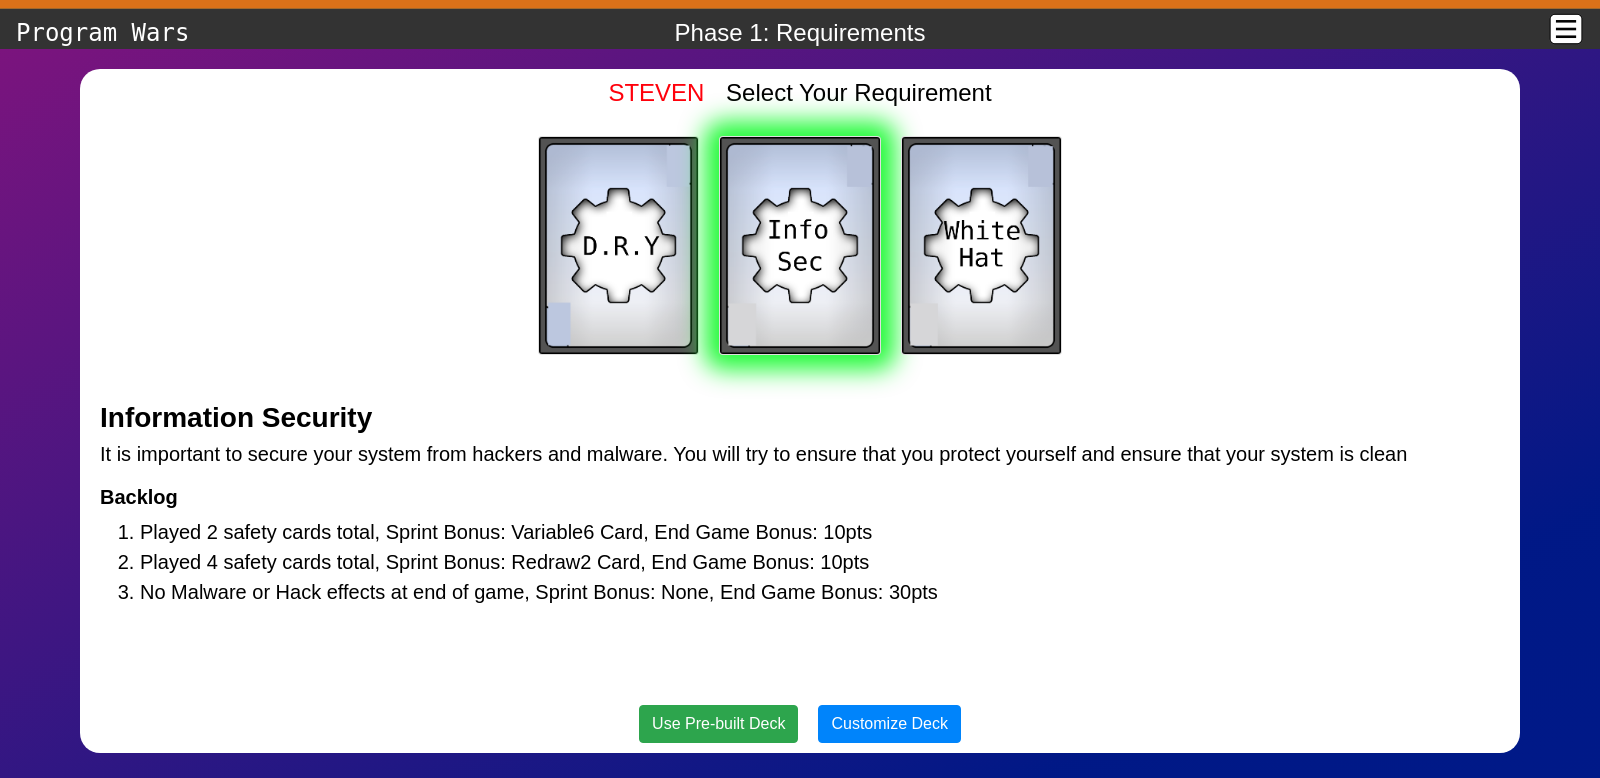
\includegraphics[width=\textwidth]{images/requirement_screen.PNG}
	\caption{The Requirements Phase Screen.}
	\label{fig:requrements}
\end{figure*}

The requirements phase allows players to pick their individual goals for the game.
These requirements are sets of individual objectives that award points and other
bonuses to the player when completed. They represent the requirements that would
be given to a developer or team by a customer for a new software project. Each
requirement has three objectives to complete during the game. Each objective is for
one of the sprints. Completing an objective by the end of the game will award the
player bonus points that will be added to their instruction score and used to determine
the winner. If a player completes an objective before the end of the sprint it is
associated with they will recieve an additional bonus. These bonuses will not be points,
but instead give the player a useful card or status effect. Some sprint bonuses may be
awarded immediately upon completing the objective and others may be awarded at the end
of the sprint, based on how they will help the player.

When players start the requirements phase they will be taken to a new page that has
the available requirements represented as cards. These cards will be on the top portion
of the screen and can be scrolled through and selected to see what their objectives are.
The bottom portion of the screen will give the conditions and bonuses granted for their
completion. When a requirements card is selected it's details will appear here. These
details will indicate the sprint the objective is related to, the bonus points for
completing the objective, and the bonus given for completing the objective before the
end of the sprint. The current prototype for this can be seen in figure???. In the future
a more diverse set of requirements will be added as well as specific card art for each
requirement.

Once a player is satisfied with the requirements they have selected they can advance to
the planning phase where they will customize a deck to help them complete their
requirements. However, an option will exist for players trying out \emph{Agile} mode,
or a new requirement, for the first time to pick a pre-built deck. If all human
players pick pre-built decks the planning phase will be skipped.

\subsection{Planning Phase}

\begin{figure*}[ht]
	\centering
	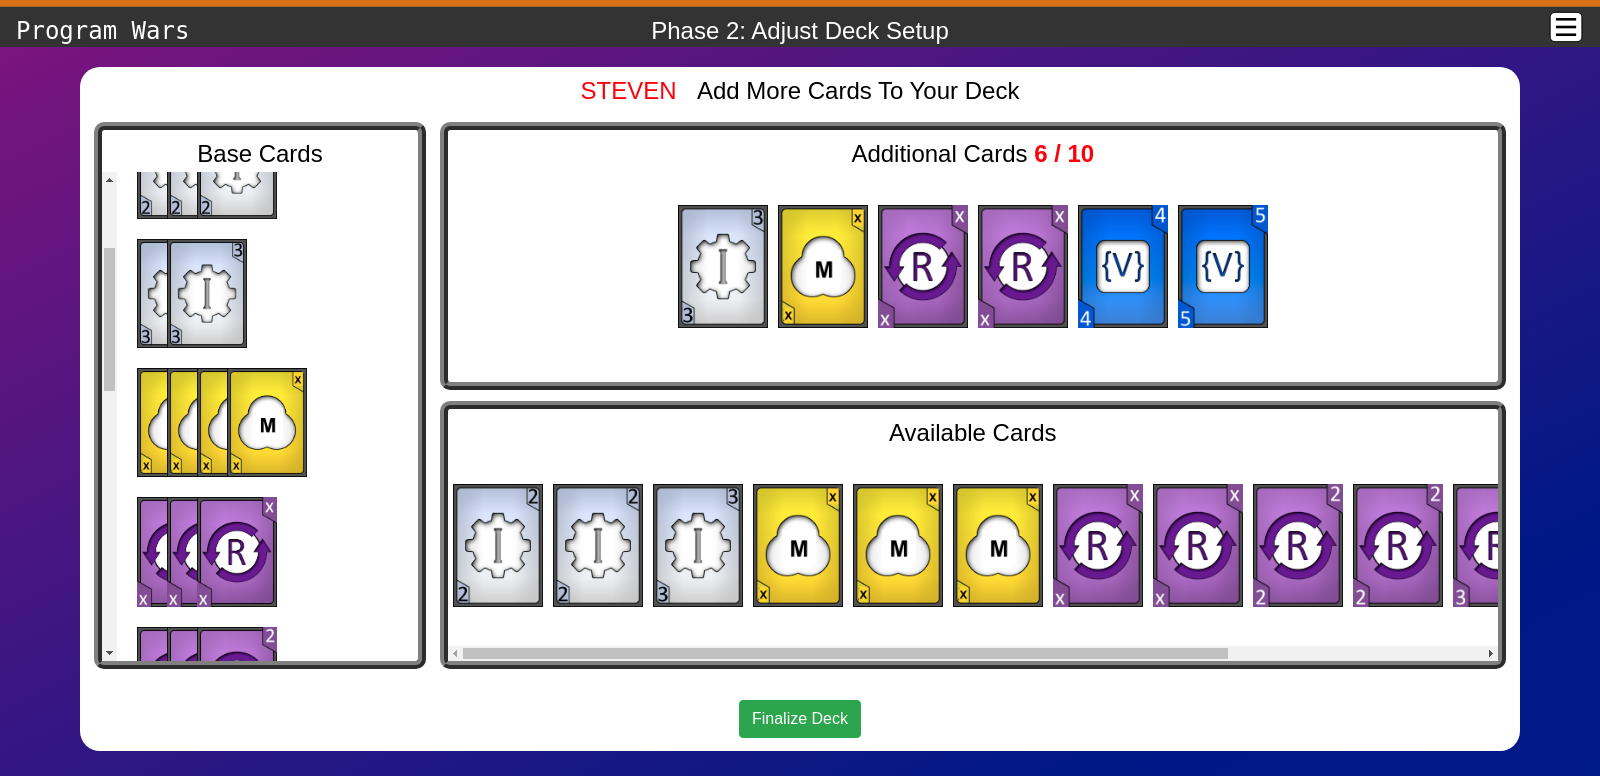
\includegraphics[width=\textwidth]{images/deck_setup_screen.PNG}
	\caption{The Planning Phase Page.}
	\label{fig:deckSetup}
\end{figure*}

Since each of the requirements has different objectives it will be necessary for
players to make some choices about how they can best complete these objectives.
The planning phase represents the part of a software project where developers
make decisions about how the software will be built and what tools they will use.
In the planning phase the player will get a base set of cards for their deck. These
cards are those that are essential for playing \gameNameNS, such as \I and \R cards.
In addition to this they will be given a pool of cards that they can choose a number
of additional cards from. The card pool will be unique to each of the requirements
so that players will have access to certain cards that are most useful for that
requirement. However, it will also have some cards that may not be essential, but
a player may still want as part of their strategy. More powerful cards will be
limited in number and will not appear in the card pools for all requirements.

When players start the planning phase they will be taken to a new page where they
can build their deck. On a portion of left side of the screen there will be a vertical
list of card types. Each type will have a pile showing how many cards of that type,
and value if applicable, will be included in the deck automatically. This way the
player knows what cards are already in their deck and can act accordingly. The rest of
the screen will be split into two horizontal lists of cards. On the top will be the
list of cards to add to the deck, and on the bottom the pool of cards the player can
pick from. Cards can be dragged between these two lists to move them around. The
upper list will have an indicator of how many cards have been added and how many
can be added total. Once a player has added the maximum number of cards to this list
they will be able to advance to the Implementation phase. If there are more than one
human players they will each be given a turn to build their deck.

\subsection{Implementation Phase}
The implementation phase is the name for the actual game in \emph{Agile} mode. For
the most part it play will be the same as it is in standard mode. The major change
is that the game no longer ends when a player reaches a specific point total. Instead
the players each get an equal number of turns through three 10 turn sprints. Once
these sprints are over the game will end. The other major change to the game play
is that completing your requirements is now a key part of winning the game. In standard
mode it is possible to ignore the bonus objectives and win the game. Generally, the
player that reaches the point total first will win. In \emph{Agile} mode the players
will need to complete at least some of their requirements in order to win the game. The
sprint bonuses will also be useful in making it easier to get more points or to
complete subsequent objectives before the end of the game. However, there may be
a set of requirements that focuses on the core aspects of the game and is less
reliant on the bonuses. This will allow beginner players an opportunity to get
used to the format without needing to excell at it immediately.

There will be some small adjustments to the game page's UI for this mode. The
first is that the score limit indicator at the top of the page will be replaced
with one that shows the current sprint and how many turns are left in it. When
a sprint is over an idicator will be given and all end of sprint bonuses that are
due will be given. All other bonuses will be given when they are completed or at
the end of the game.

Second the player information panel will no longer need a score meter. Since there
is no points total to progress toward the score meter and the current score display
will not be useful. They will be replaced with a simple indicator showing the
players instructions score. It will also be useful to have some kind of compact
indicator for the players progress toward the current sprint's objective. For example,
if the player's objective is to build two card stacks that both have nested
loops\footnote{A card stack with two \R cards on it.} the indicator could say
``Nested Loops: 0/2" and update as they built these stacks. This would reduce
the context switching the player would need to do during the game to keep track of
their requirements.

Lastly, in order to allow the player to see a more detailed view of their set of
requirements, a new tab will be added. This replace the standard mode bonus tab.
This tab will show a player each of the sprint objectives they need to complete
as well as any rewards they will receive for completeing them. Like the current
bonus tab awarded bonuses can change color to indicate that they have been given
to the player. There can also be clear indicators of progress for each objective.

When all three sprints have ended the game will advance to the testing phase.

\subsection{Testing Phase}
The testing phase is a replacement for the winner's modal that is displayed at
the end of beginner and standard modes. This phase represents a kind of acceptance
testing phase for the program the player built. The player had requirements to
fulfill for the project so they are judged on their progress. This is where the
bonus points for requirements will be added to a player's instruction score. The
detailed progress for each player toward their requirements will be shown. Here
human players will be able to see how close an AI player came to completing their
requirements. The player with the most points will be the winner. Tie breaks will
favour the player that completed more requirements in total or by the end of the
appropriate sprint. The points given for requirements should be balanced to allow
strategies that do not focus as much on instruction score to be competetive if
they are completed.



\section{Game Cards}
The player builds their program using the basic building blocks of instructions, methods and repetition. Also, on their turn, a player can launch a cyberattack at an opponent or prepare their defence. This section describes each of the computer programming, cyberattack and cybersecurity cards in the game.

\subsection{Computer Programming}
In \pwOne the majority of cards focused on computer programming concepts, and most of these cards carry over into \pwThree. 

\paragraph{\Ins, \R and \Vns:}As in actual computer programs, instructions form the backbone of the program. The \I card represents a fixed number of instructions (1, 2, or 3) and the player uses this type of card as the basis for gaining points in the game. Players can then use the \R card, which represents the concept of a loop, to further increase the overall number of instructions in their program. There are three sizes of \R cards: 2, 3, and 4. By placing a \R card on another \R card, the player can form a nested loop.\footnote{\gameName only allows nesting up to two levels to reduce the gameplay complexity and to keep scores from growing too quickly.} In addition to the fixed-size \R cards, there is also a variable \R card (called \Rxns). By itself, this card acts as a \Rns-1 card. However, the player can place a \V card on a \Rx to increases its multiplicative power. \V cards have values of 3, 4, 5 and 6. 

%Figure \ref{fig:game} shows the example where a \M card, \R card and \V card are used.

\paragraph{\Mns:}
In \pwOneNS, the \Gr card represented the concept of a procedure, function or method in a programming language. However, the user study of \pwOne showed this card to be ineffective in conveying this concept. \pwThree\\ replaces the \Gr card with the \M card to address this problem.

The \M card acts as a proxy for the contents of the \MS area, with the player's total score being adjusted accordingly. If a new card is added to the \MS area, the player's score will be adjusted according to the number of \M cards in the \Play area.
As with \I cards, the player can use \R and \V cards to increase the effect of a \M card. 

\subsection{Malware}
\label{section:malware}

\pwOne represented the malware cyberthreat with a single \Mal card. In \pwThree, the \Mal card is replaced with cards that more directly represent four of the most common types of malware: \Spyns, \Ranns, \Vi and \Trjns. 

Spyware is used to gather and send information to another party without the target’s consent. The \Spy card represents this same situation in the context of the game. Ransomware is used for collecting a specific points from the targeted player. The \Vi card is used to reduce the effect of a stack of cards in the \Play area by reducing the points of a card stack and the \Trj card is played against an opponent, as a random card in the opponent's hand which replaced with one that mimics it.

\begin{comment}

\paragraph{\Spyns:}
Spyware is used to gather and send information to another party without the target’s consent. The \Spy card represents this same situation in the context of the game. When a player plays a \Spy card against their opponent, a button labelled ``Spy Hand'' appears beside the opponent's name in the top portion of the screen. Clicking this button allows the attacker to be able to see the affected player's hand. The effect lasts for five turns.

\paragraph{\Ranns:}
This card's effect reflects the real-world concept of ransomware where an attacker blocks access to a target's files, such as encrypting them, and threatens to publish or delete them unless a ransom is paid. When a player plays a \Ran card on an opponent, the targeted player loses 10 points from their total score and these points are added to the attacker's score. This can result in an opponent's score becoming negative. Unlike real-world ransomware, recovering from this attack is simple, as an affected player can recover their points by either using a \Scan or \Anti card. 

\paragraph{\Vins:}
A computer virus is a computer program that replicates itself by modifying other programs. The \Vi card is used to reduce the effect of a stack of cards in the \Play area by reducing the points of a card stack. If the stack is built on an \I card, the stack's score becomes 0. If the stack is built on a \M card, the stack's score is reduced by 50\%. This adds additional motivation for the player to use the \M card. This card is the most similar to the \Mal card from \pwOneNS, where the \Mal card reduced a player's total score by 25\%.   

\paragraph{\Trjns:}
In the real world, a \Trj is a computer program that misleads users as to its real intent. When a \Trj card is played against an opponent, a random card in the opponent's hand is replaced with one that mimics it. While players can see when a \Trj is played on them they cannot tell which card has been mimicked. The actual effect of the mimic card depends on what card is replaced. \I and \M cards add the \Buf effect to the player instead of creating a new stack in the \Play area. \R and \V cards add a \Vi card to the stack where they were added. Cyberattack cards, such as \DoS or \Vins, add a \CSS to the player instead of adding a cyberattack effect to the target opponent. All cybersecurity and algorithm cards add a \Ran to the player instead of activating the expected card.

\end{comment}

\subsection{Hacking}
\label{section:hacking}
\pwOne contained a single card, \Hackns, that represented an intrusion into a computer system. The effect of the \Hack card was to remove one of the stacks of cards on an opponent's playfield. \pwThree refines this idea by adding specific cards to represent common ways whereby computer systems are intruded or affected by an intrusion. These four cards provide representations of the effects of four types of system attacks: causing a buffer overflow, cross-site scripting, a denial of service attack (DoS), and injection of malicious SQL code.

The \Buf card prevents an opponent from playing any \Ins, \Rns, \V or \M cards for two turns. The \CSS card stops a player from playing any algorithm or cyberattack cards for two turns. \DoS card prevents a player from redrawing new cards at the end of their turn and finally the \SQL card can be used to slow down the progress of an opponent by reducing the total of the \MS area by two points.

\begin{comment}

\paragraph{\Bufns:}
A common system attack is to send data to a program such that a memory buffer overflows and cause program instructions to be overwritten by malicious code, which is then run. In \pwTwoNS, the \Buf card prevents an opponent from playing any \Ins, \Rns, \V or \M cards for two turns. During this effect a \emph{Pass} button is added next to the \emph{Redraw} button. This allows a player to skip their turn if they cannot play any cards and do not want to discard one. The concept behind this card's effect is similar to real-world buffer overflow solutions \cite{libsafe, StackGuard}.

\paragraph{\CSSns:}
Cross-site scripting is a code injection attack. The attack happens when the victim visits a web page or web application that administers the harmful code \cite{Crosssite}. The visited web page or service acts as a carrier to deliver the malicious code to the affected browser. In \pwTwoNS, the \CSS card stops a player from playing any algorithm or cyberattack cards for two turns. This effect also adds a \emph{Pass} button above the \Hand. The concept behind this card is to make a player familiar with this type of attack by preventing the advantages given by algorithm and cyberattack cards.

\paragraph{\DoSns:}
A Denial of Service (DoS) attack occurs when a computer system connected to a network is intentionally flooded with requests so that the system can no longer handle legitimate requests. In \pwTwoNS, the \DoS card prevents a player from redrawing new cards at the end of their turn. The effect also adds a \emph{Pass} button above the \Hand~ and disables the \emph{Redraw} button. The effect lasts for three turns resulting in the player having fewer cards in their hand to choose from until the effect ends.

\paragraph{\SQLns:}
In an SQL injection attack, malicious SQL code is entered into a data field such that the code is run on a backend database. The result of such an attack is to obtain information that was not intended to be disclosed or delete and/or corrupt the data in the database. In \pwTwoNS, the \SQL card can be used to slow down the progress of an opponent by reducing the total of the \MS area by two points. The effect lasts until removed by a \Fire or \Scan card. The concept behind this card is that of infiltration of a program's method by malicious code. 

\end{comment}

\subsection{Cyberdefense:}
\pwOne provided three cards for cyberdefense. Two of the cards were \emph{permanent} cards, meaning that they remained on a player's playfield when played, and were referred to as \emph{Safeties}. The first of these cards was the \Anti card which prevented the \Mal card from being played on a player. The second of these cards was the \Fire card which protected against the \Hack card. The third card was the \Over card, which combated the \Mal card by increasing the player's total score by 25\%. However, it was observed that the \Over effect didn't match well with real-world cybersecurity concepts and was removed in \pwThree.  

\pwThree continues the use of the two safety cards, \Anti and \Firens, and adds a new one-time-use cyberdefense card called \Scanns. 

The \Scan card represents the action of a user explicitly scanning all of their files to find any infected items using an antivirus tool. The \Anti card reflects this real-world tool by protecting a player from the effect of any of the malware attack cards. \Fire card prevent hack cards being played on the player.

\begin{comment}

\paragraph{\Scanns:}
The \Scan card represents the action of a user explicitly scanning all of their files to find any infected items using an antivirus tool. If the player is under the influence of either a malware or a hack card, then the \Scan card allows the players to choose a single effect to remove. If the player is not under the influence of a cyberattack card, the effect is saved until the player is attacked, at which time the cyberattack is neutralized and the \Scan effect is removed. 

\paragraph{\Antins:}
An antivirus program is a program or set of programs designed to prevent, search for, detect, and remove malware from a computer system. The \Anti card reflects this real-world tool by protecting a player from the effect of any of the malware attack cards. If the player is already under the effect of one or more malware cards, all of the effects are removed when this card is played. Unlike the \Scan card, the effect of this card is permanent once it is played, thereby protecting the player from any future malware card attacks. 

\paragraph{\Firens:}
A firewall is a network security device that controls incoming and outgoing network traffic and grants or prevents data packets based on a set of security rules, thereby protecting a computer system from various intrusion attacks. Like the \Anti card, the \Fire card reflects this real-world tool by preventing hack cards from being played on the player. Similar to the \Anti card, if the player is affected by any hack cards, these effects are removed. The effect of this card is also permanent once played.

\end{comment}

\subsection{Algorithms/Library Functions:}
The use of algorithms, often from libraries, is an essential part of computer programming. Two key categories of algorithms are searching and sorting, and both of these are introduced in \pwThree.

The \Sort card allows a player to rearrange the top five (5) cards of the deck into whatever order they choose and the \Ser card allows a player to search for a specific card within the top ten (10) cards of the deck.

\begin{comment}

\paragraph{\Sortns:}
Sorting is the arrangement of items into an ordered sequence. In \pwTwoNS, the \Sort card allows a player to rearrange the top five (5) cards of the deck into whatever order they choose. This allows a player to control what cards players will draw for the next five turns, three cards for the player, and two for their opponent. When the card is played, an overlay is opened showing the top five cards and the player can drag and drop cards to reorder them.

\paragraph{\Serns:}
Searching is the process of locating a particular element in a given set of elements. In \pwTwoNS, the \Ser card allows a player to search for a specific card within the top ten (10) cards of the deck. Playing the card results in an overlay being opened that shows these cards and the player selects one to immediately put into their hand for their next turn.

\end{comment}
\section{Conclusion}
Nee to re-write
\section{Acknowledgements}
Need to re-write

\bibliographystyle{ACM-Reference-Format}
\balance
\bibliography{paper_JSEET_2021}

\end{document}
